\documentclass{article}\usepackage[]{graphicx}\usepackage[]{color}
% maxwidth is the original width if it is less than linewidth
% otherwise use linewidth (to make sure the graphics do not exceed the margin)
\makeatletter
\def\maxwidth{ %
  \ifdim\Gin@nat@width>\linewidth
    \linewidth
  \else
    \Gin@nat@width
  \fi
}
\makeatother

\definecolor{fgcolor}{rgb}{0.345, 0.345, 0.345}
\newcommand{\hlnum}[1]{\textcolor[rgb]{0.686,0.059,0.569}{#1}}%
\newcommand{\hlstr}[1]{\textcolor[rgb]{0.192,0.494,0.8}{#1}}%
\newcommand{\hlcom}[1]{\textcolor[rgb]{0.678,0.584,0.686}{\textit{#1}}}%
\newcommand{\hlopt}[1]{\textcolor[rgb]{0,0,0}{#1}}%
\newcommand{\hlstd}[1]{\textcolor[rgb]{0.345,0.345,0.345}{#1}}%
\newcommand{\hlkwa}[1]{\textcolor[rgb]{0.161,0.373,0.58}{\textbf{#1}}}%
\newcommand{\hlkwb}[1]{\textcolor[rgb]{0.69,0.353,0.396}{#1}}%
\newcommand{\hlkwc}[1]{\textcolor[rgb]{0.333,0.667,0.333}{#1}}%
\newcommand{\hlkwd}[1]{\textcolor[rgb]{0.737,0.353,0.396}{\textbf{#1}}}%
\let\hlipl\hlkwb

\usepackage{framed}
\makeatletter
\newenvironment{kframe}{%
 \def\at@end@of@kframe{}%
 \ifinner\ifhmode%
  \def\at@end@of@kframe{\end{minipage}}%
  \begin{minipage}{\columnwidth}%
 \fi\fi%
 \def\FrameCommand##1{\hskip\@totalleftmargin \hskip-\fboxsep
 \colorbox{shadecolor}{##1}\hskip-\fboxsep
     % There is no \\@totalrightmargin, so:
     \hskip-\linewidth \hskip-\@totalleftmargin \hskip\columnwidth}%
 \MakeFramed {\advance\hsize-\width
   \@totalleftmargin\z@ \linewidth\hsize
   \@setminipage}}%
 {\par\unskip\endMakeFramed%
 \at@end@of@kframe}
\makeatother

\definecolor{shadecolor}{rgb}{.97, .97, .97}
\definecolor{messagecolor}{rgb}{0, 0, 0}
\definecolor{warningcolor}{rgb}{1, 0, 1}
\definecolor{errorcolor}{rgb}{1, 0, 0}
\newenvironment{knitrout}{}{} % an empty environment to be redefined in TeX

\usepackage{alltt}
\usepackage{Sweave}
\usepackage{float}
\usepackage{graphicx}
\usepackage{tabularx}
\usepackage{siunitx}
\usepackage{mdframed}
\usepackage{natbib}
%\bibliographystyle{..//papers/styles/besjournals.bst}
\usepackage[small]{caption}
\setkeys{Gin}{width=0.8\textwidth}
\setlength{\captionmargin}{30pt}
\setlength{\abovecaptionskip}{0pt}
\setlength{\belowcaptionskip}{10pt}
\topmargin -1.5cm        
\oddsidemargin -0.015cm   
\evensidemargin -0.015cm
\textwidth 16cm
\textheight 21cm 
%\pagestyle{empty} %comment if want page numbers
\parskip 7.2pt
\renewcommand{\baselinestretch}{2}
\parindent 20pt
\usepackage{indentfirst} 

\newmdenv[
  topline=true,
  bottomline=true,
  skipabove=\topsep,
  skipbelow=\topsep
]{siderules}
\IfFileExists{upquote.sty}{\usepackage{upquote}}{}
\begin{document}

\renewcommand{\thetable}{\arabic{table}}
\renewcommand{\thefigure}{\arabic{figure}}
\renewcommand{\labelitemi}{$-$}

\renewcommand{\thesection}{\arabic{section}.}
\renewcommand\thesubsection{\arabic{section}.\arabic{subsection}} 

%%%%%%%%%%%%%%%%%%%%%%%%%%%%%%%%%%%%
\section*{Exploring model accuracy using weather station vs hobo logger data}

\large{\textbf{Key Points:}
\begin{enumerate}
\item By accounting for microclimates, we improve model accuracy in predicting leafout (Figure \ref{fig:compare})
\item Individuals that leaf out later grow less over the course of a season (Figure \ref{fig:cg})
  \begin{enumerate}
  \item Additionally, individuals from more northern provenance latitudes grow less (Figure \ref{fig:cg})
  \end{enumerate}
\item Thus, it is crucial to improve model accuracy for predicting leafout in order to better understand temperate forest growth in the face of climate change. 
\item Additionally, accounting for microclimates improves model prediction for growing degree days (GDDs) from budburst to leafout, which is essential for understanding false spring risk (Figure \ref{fig:dvr})
\item Finally, using phenology observations for the Arnold Arboretum (2015-2019), Harvard Forest (2015-2018) and a common garden (2017-2019) we see that, overall, there is variation across sites in GDDs to leafout (Figure \ref{fig:allsites}). 
  \begin{enumerate}
  \item The common garden site -- which was planted in 2016 -- initiated leafout with fewer GDDs than the Arboretum and Harvard Forest required more GDDs for leafout to occur, but provenance latitude has little affect on GDDs to leafout. 
  \end{enumerate}
\end{enumerate}

{\begin{figure} [H]
  -\begin{center}
  -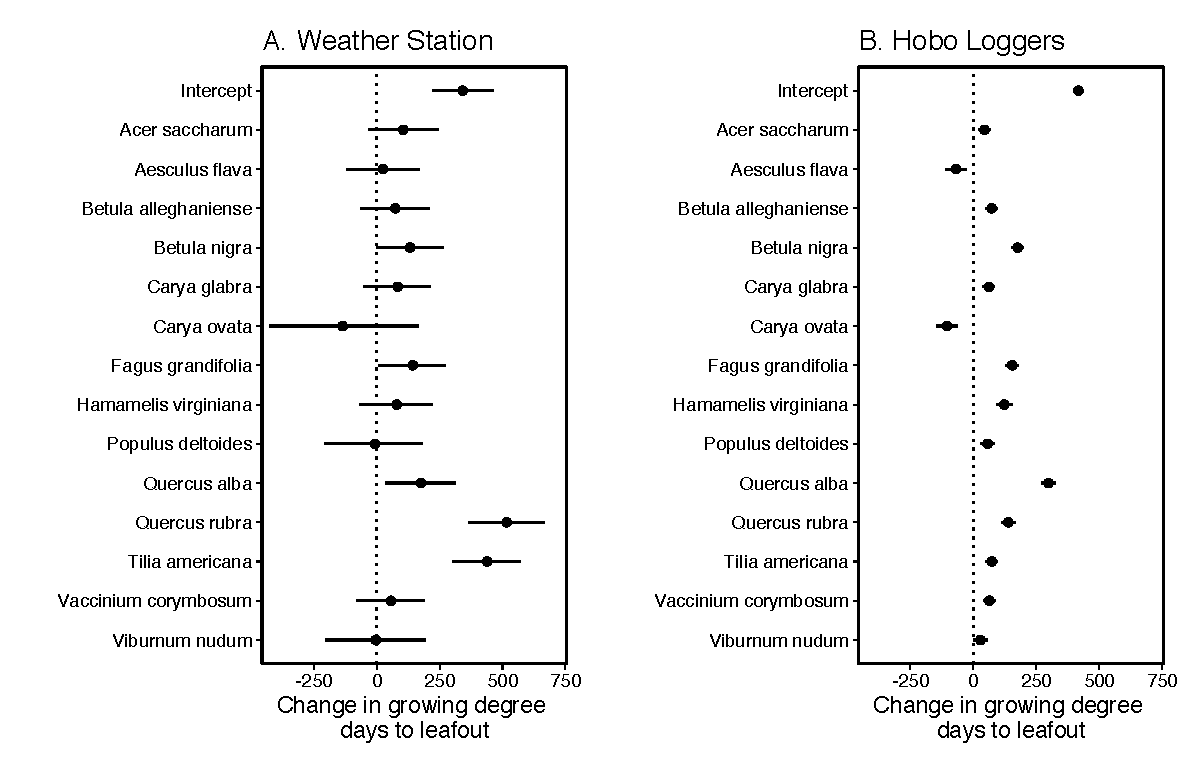
\includegraphics[width=16cm]{..//analyses/figures/muplot_compare_lo.pdf}
  -\caption{Model output for growing degree days to leafout using weather station data (A) and hobo logger data (B). Dots and lines show means and 50\% uncertainty intervals.}\label{fig:compare}
  -\end{center}
  -\end{figure}}
  
{\begin{figure} [H]
  -\begin{center}
  -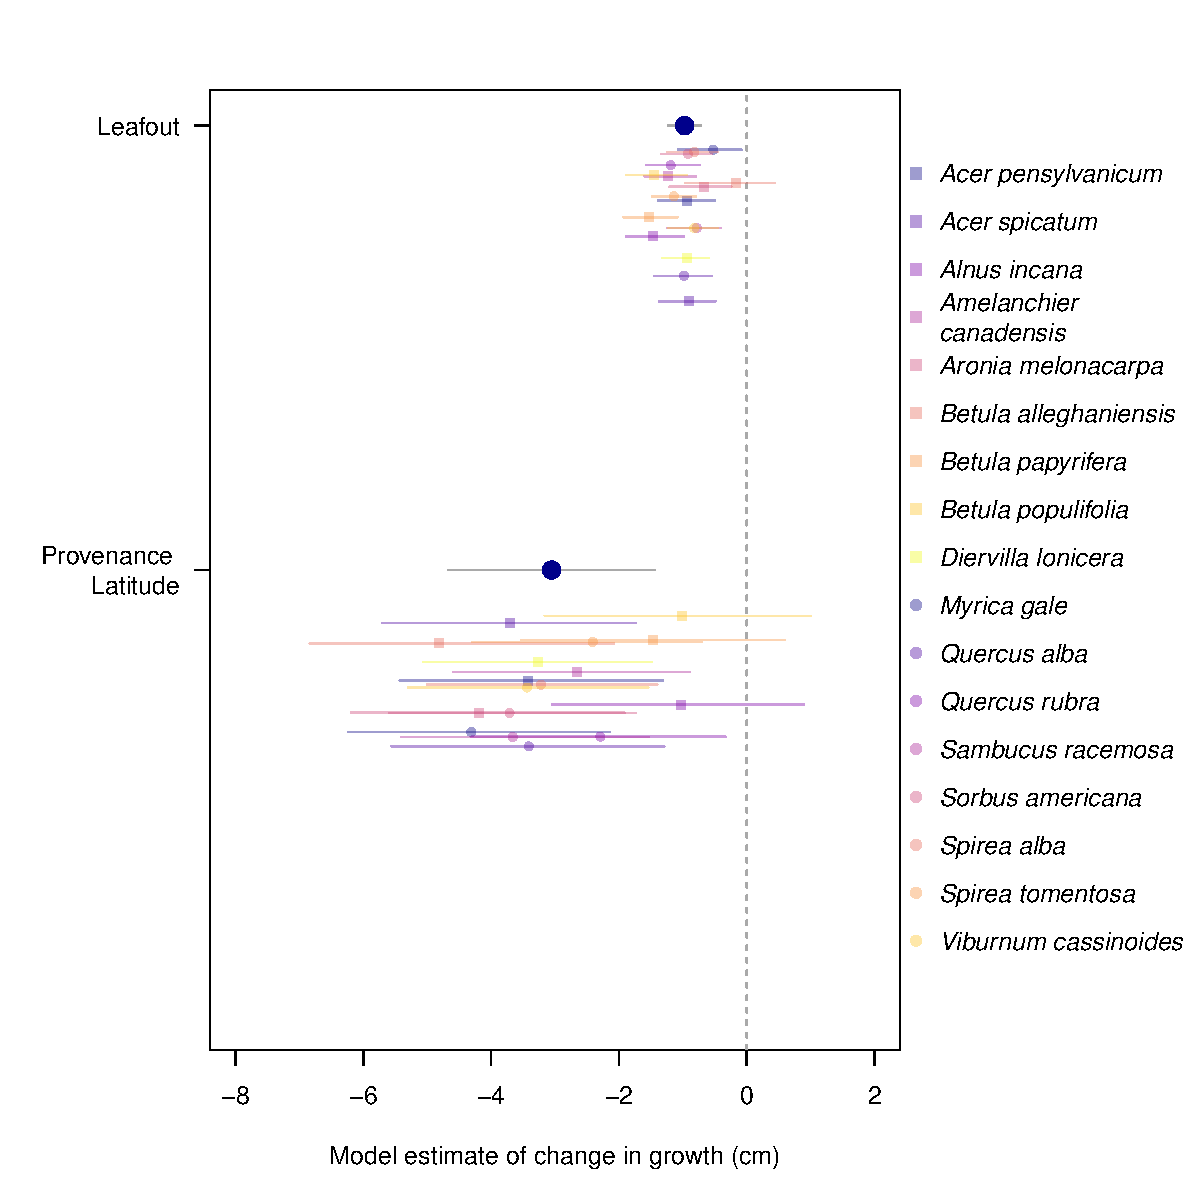
\includegraphics[width=12cm]{..//analyses/figures/cg_height.pdf}
  -\caption{Model output for amount of growth over a season (cm). Dots and lines show means and 50\% uncertainty intervals.}\label{fig:cg}
  -\end{center}
  -\end{figure}}

{\begin{figure} [H]
  -\begin{center}
  -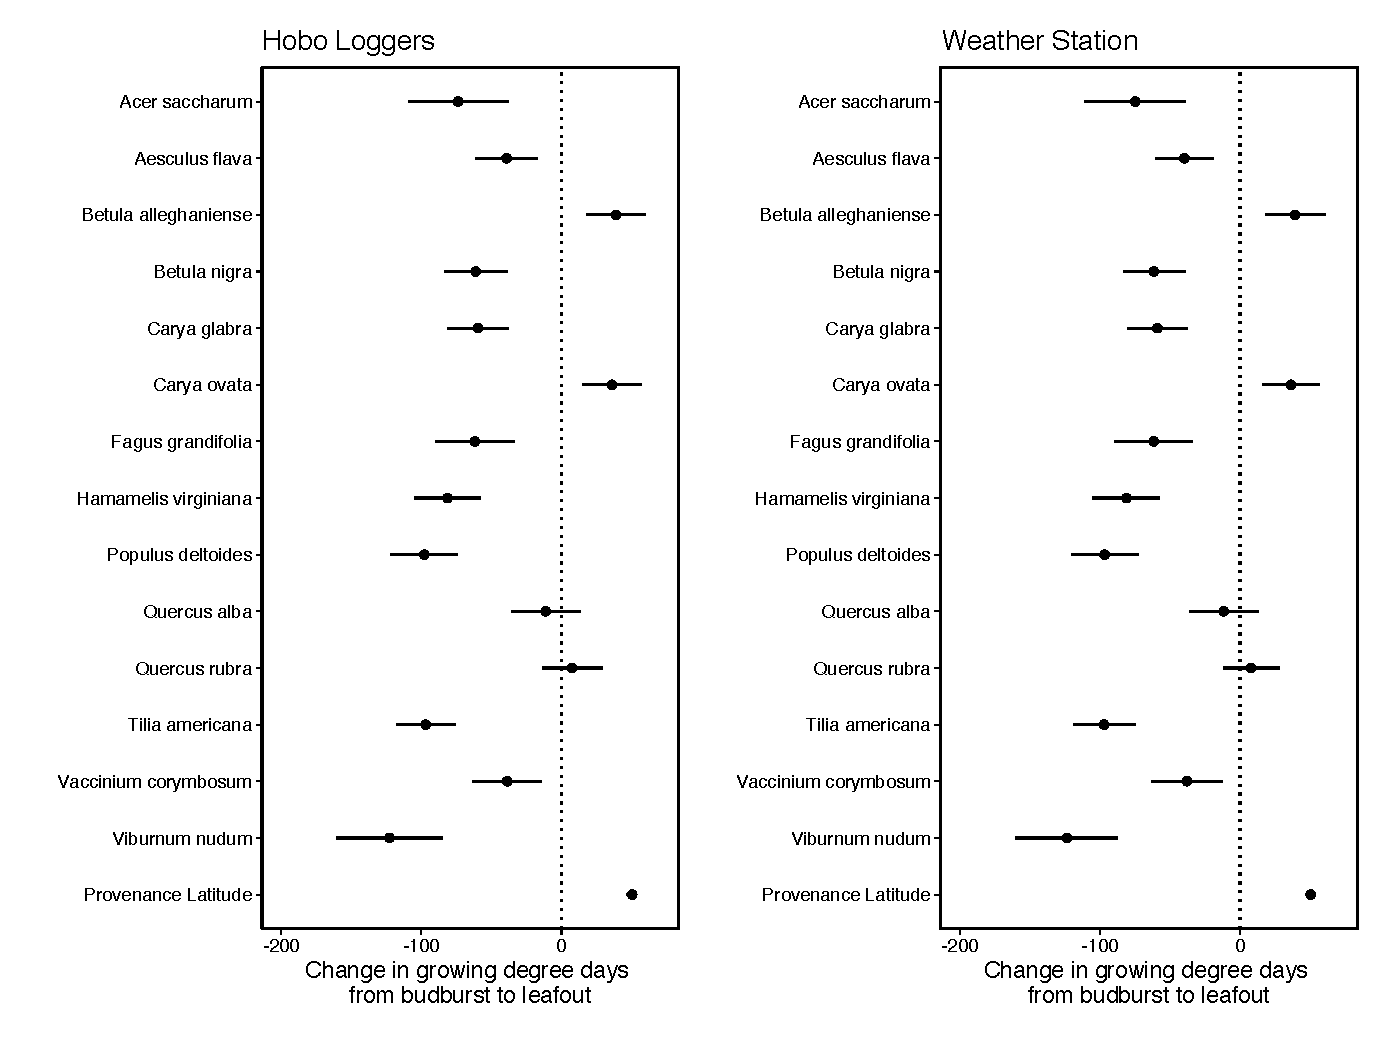
\includegraphics[width=16cm]{..//analyses/figures/muplot_compare_dvr.pdf}
  -\caption{Model output for growing degree days from budburst to leafout using weather station data (A) and hobo logger data (B). Dots and lines show means and 50\% uncertainty intervals. Note the x-axis scales are differently to see the estimates more clearly.}\label{fig:dvr}
  -\end{center}
  -\end{figure}}
  
{\begin{figure} [H]
  -\begin{center}
  -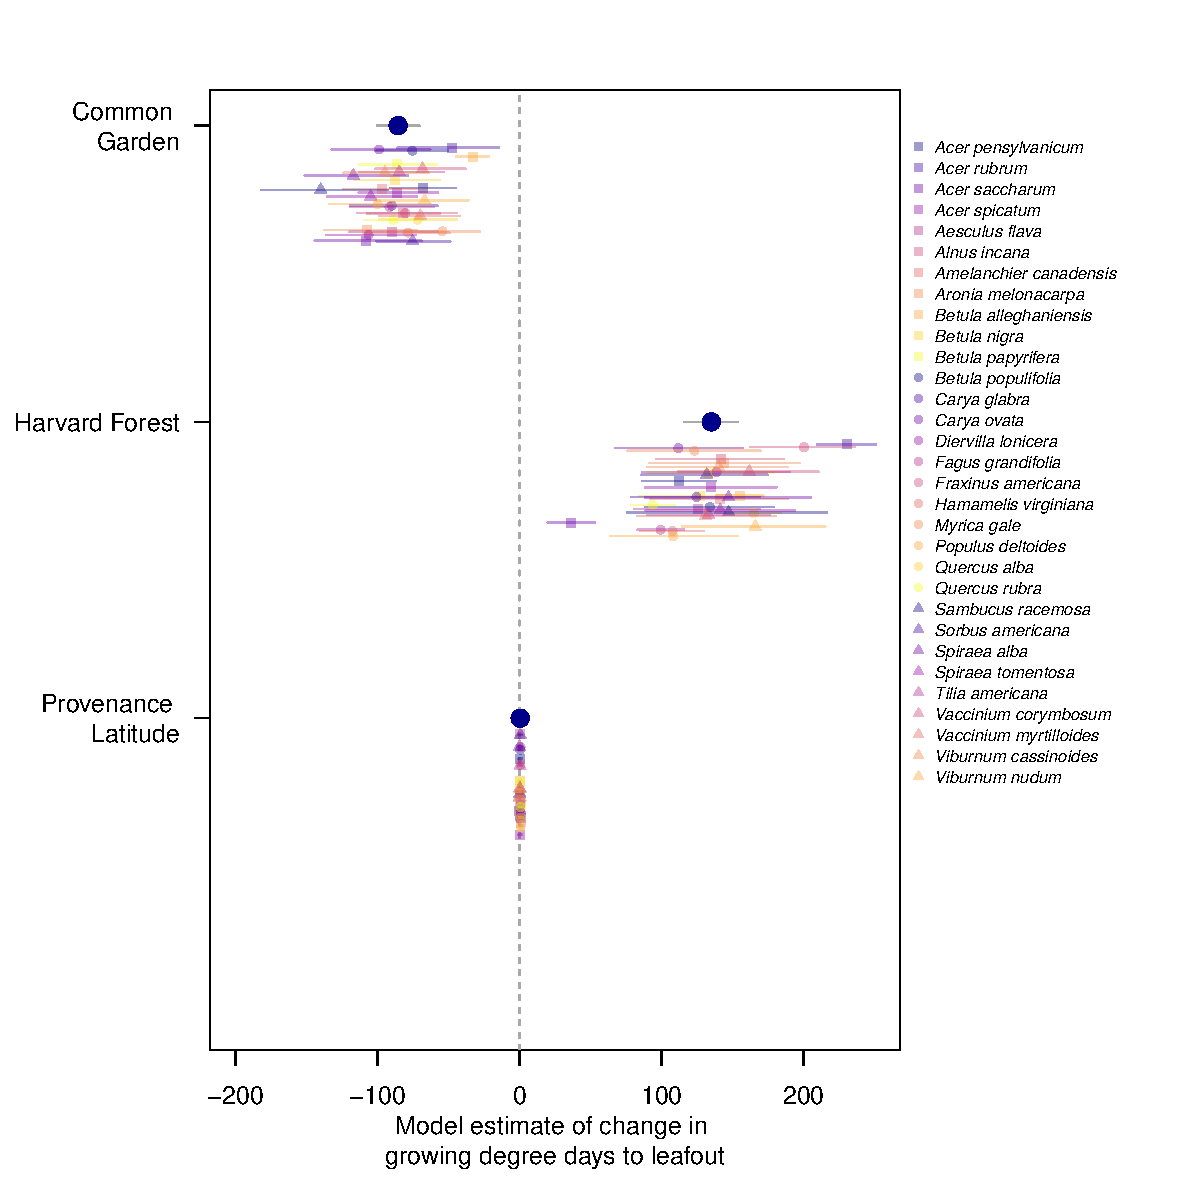
\includegraphics[width=12cm]{..//analyses/figures/site_prov_all.pdf}
  -\caption{Model output for growing degree days to leafout using weather station data comparing three different sites. The Arnold Arboretum is the intercept. Dots and lines show means and 50\% uncertainty intervals.}\label{fig:allsites}
  -\end{center}
  -\end{figure}}

\section*{Supplemental figures}

{\begin{figure} [H]
  -\begin{center}
  -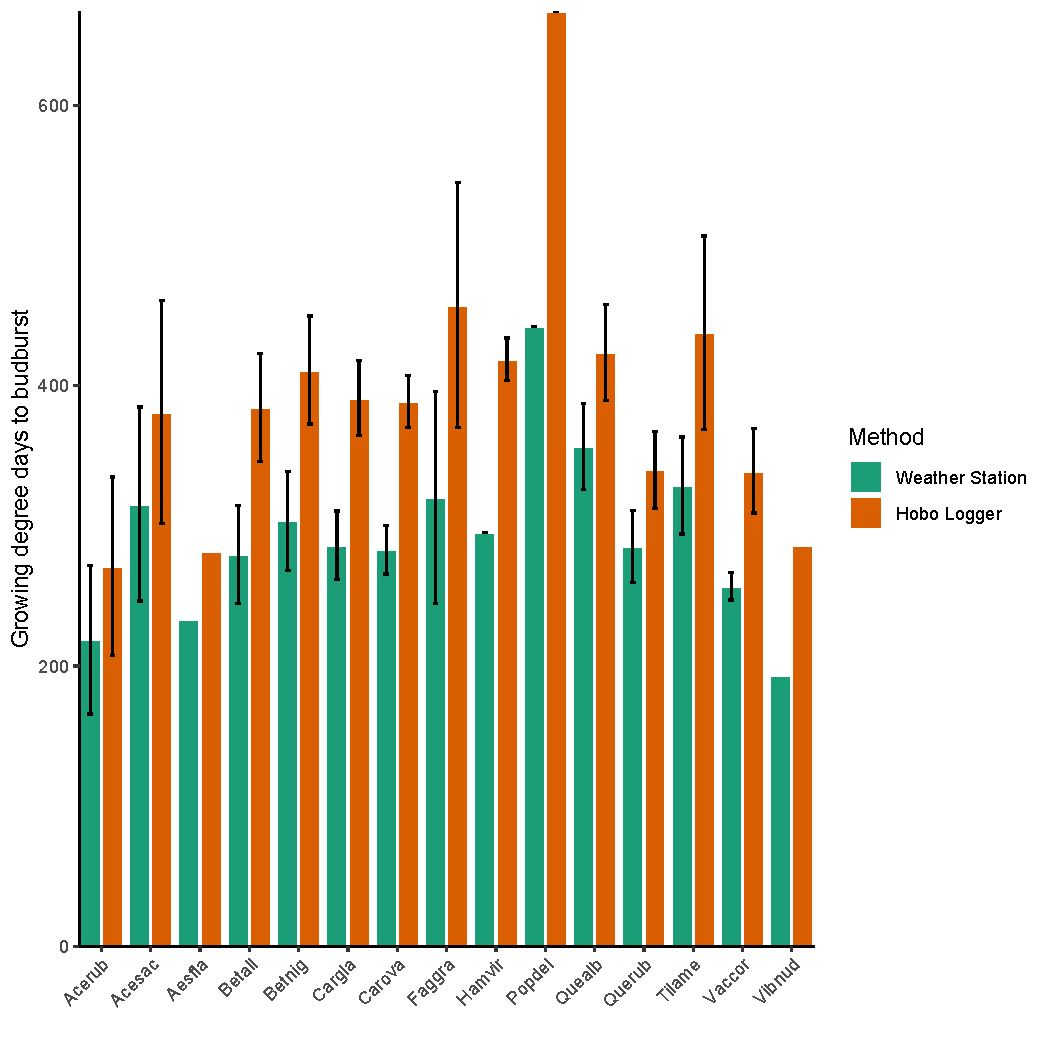
\includegraphics[width=12cm]{..//analyses/figures/stationvshobo_ts2019.pdf}
  -\caption{}\label{fig:barcompare}
  -\end{center}
  -\end{figure}}
  
{\begin{figure} [H]
  -\begin{center}
  -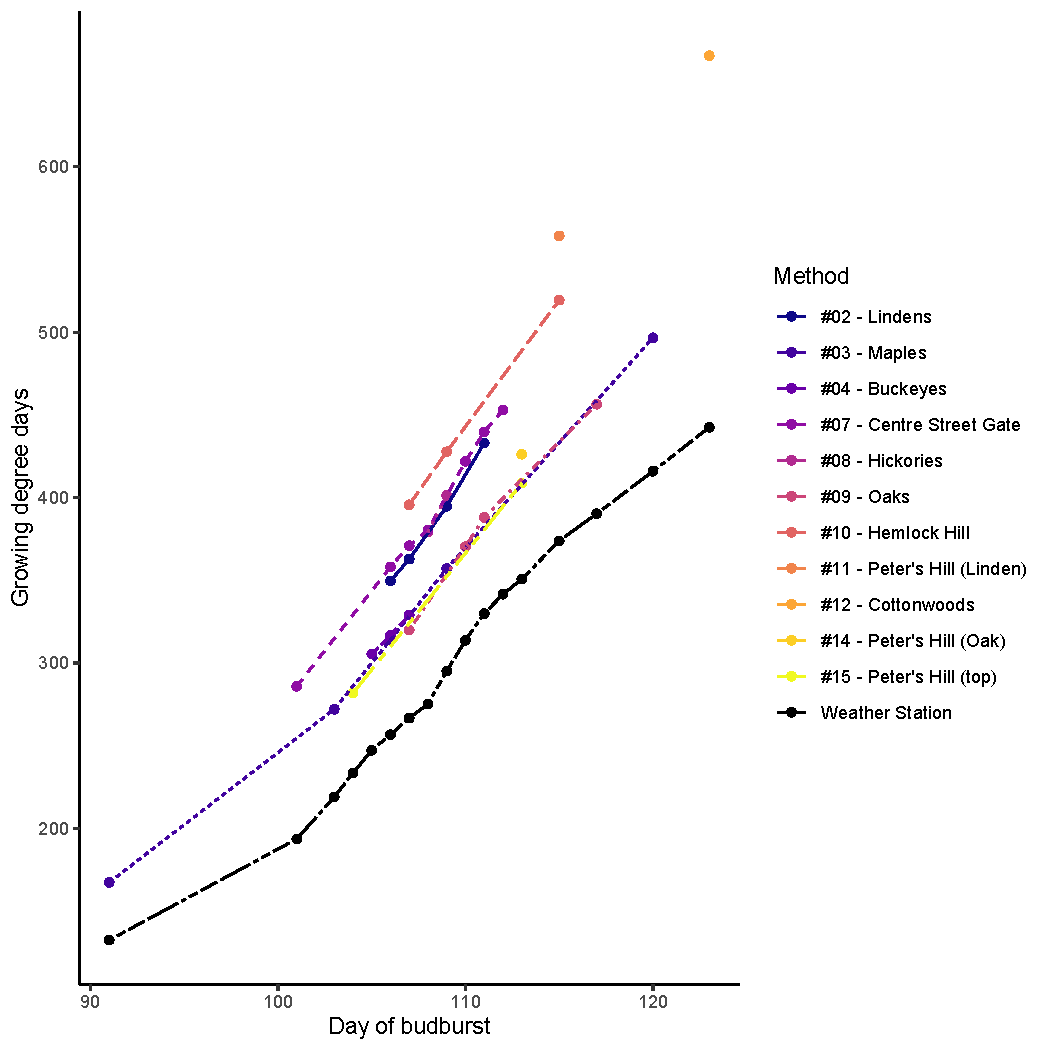
\includegraphics[width=12cm]{..//analyses/figures/loggerbreakdown.pdf}
  -\caption{}\label{fig:loggers}
  -\end{center}
  -\end{figure}}

\end{document}
